\documentclass[11pt]{article}

% 页面设置
\usepackage[top=1cm, bottom=2cm, left=1cm, right=1cm]{geometry}

% 中文支持
\usepackage{ctex}

% 数学包
\usepackage{amsmath, amssymb, amsthm}

% 算法包
\usepackage[linesnumbered, ruled]{algorithm2e}

% 颜色和命令定义
\usepackage{xcolor, xparse}

% 代码显示
\usepackage{listings}

% 图形包
\usepackage{graphicx}

% 子图包
\usepackage{subcaption}

% 表格包
\usepackage{booktabs}

% 其他需要的包
\usepackage{mathrsfs}
\usepackage{wrapfig}
\usepackage{forest}
\usepackage[normalem]{ulem} % 保持 \emph 为斜体
\usepackage{bm}
\usepackage{multicol}
\usepackage{verbatim}
\usepackage{float}
\usepackage{pifont}

% 添加 'soul' 包用于高亮和支持换行
\usepackage{soul}

% 定义自定义颜色
\definecolor{cmdbg}{RGB}{220, 220, 220} % 浅灰色背景

% 设置高亮颜色
\sethlcolor{cmdbg}

% 定义 \ccmd 命令,用于行内代码片段
\newcommand{\ccmd}[1]{\texttt{\hl{#1}}}

% 超链接(放在最后)
\usepackage[colorlinks=true, linkcolor=blue]{hyperref}

\author{
    \makebox[0.8\textwidth]{%
        \centering
        杨远青 \quad 22300190015 \quad
        \href{https://github.com/bud-primordium/Computational-Physics-Fall-2024}{\raisebox{-2pt}{
\includegraphics[height=12pt]{../.utils/comphys.pdf}}}
    }
}



\title{计算物理作业6}

\begin{document}
\maketitle
\textit{起视四境,而作业又至矣。}
\section{题目 1:一维 Kronig-Penney 模型的本征值求解}
\subsection{题目描述}
\noindent Write a code to numerically solves the motion of a simple pendulum using \textbf{Euler's method, midpoint method, RK4 method} and \textbf{Euler-trapezoidal method} (implement these methods by yourself). Plot the angle and total energy as a function of time. Explain the results.

\subsection{程序描述}
本程序内置了一个Pendulum类,具有绳长,质量(小球视作质点),初始角度,初始角速度,重力加速度等属性。通过调用Pendulum类的方法,可以使用Euler's method, midpoint method, RK4 method和Euler-trapezoidal method来求解简单摆的运动,会返回角度与角速度的numpy数组。类的方法还包括辅助的导数计算,即演化方程
\[
\begin{aligned}
\frac{d\theta}{dt} &= \omega, \\
\frac{d\omega}{dt} &= -\frac{g}{L} \sin(\theta),
\end{aligned}
\]
与总能量采集方法
\[
E = T + V = \frac{1}{2} m (\omega L)^2+ m g L (1 - \cos\theta)
\]
主程序还有内置的解析解、误差计算与用户输入采集函数,其中解析解借助了\texttt{scipy.special}的雅可比椭圆积分\texttt{sn,cn},模数$k = \sin(\theta_0/2)$,固有频率$\omega_0 = \sqrt{\frac{g}{L}}$,所以对大角度的摆动也是精确的。
\[
\theta(t) = 2 \arcsin\left(k \, \text{sn}(\omega_0 t + \frac{\pi}{2}, k^2)\right)
\]
\[
\omega(t) = \frac{2 k \omega_0 \, \text{cn}(\omega_0 t + \frac{\pi}{2}, k^2)}{\sqrt{1 - k^2 \, \text{sn}^2(\omega_0 t + \frac{\pi}{2}, k^2)}}
\]

\subsubsection{欧拉法 (Euler’s Method)}

\[
\begin{aligned}
\theta_{i+1} &= \theta_i + h \cdot \frac{d\theta}{dt} \bigg|_{t_i} \quad
\omega_{i+1} = \omega_i + h \cdot \frac{d\omega}{dt} \bigg|_{t_i}
\end{aligned}
\]

\subsubsection{中点法 (Midpoint Method)}

\[
\begin{aligned}
\text{计算中点值:} \quad
\theta_{\text{mid}} &= \theta_i + \frac{h}{2} \cdot \frac{d\theta}{dt} \bigg|_{t_i}, \quad
\omega_{\text{mid}} = \omega_i + \frac{h}{2} \cdot \frac{d\omega}{dt} \bigg|_{t_i} \\
\text{使用中点斜率更新:} \quad
\theta_{i+1} &= \theta_i + h \cdot \frac{d\theta}{dt} \bigg|_{\text{mid}}, \quad
\omega_{i+1} = \omega_i + h \cdot \frac{d\omega}{dt} \bigg|_{\text{mid}}
\end{aligned}
\]

\subsubsection{四阶龙格-库塔法 (RK4 Method)}

\[
\begin{aligned}
\text{第一步 (\(k_1\)):} \quad
k_1^\theta &= \frac{d\theta}{dt} \bigg|_{t_i, \theta_i, \omega_i}, \quad
k_1^\omega = \frac{d\omega}{dt} \bigg|_{t_i, \theta_i, \omega_i}; \\
\text{第二步 (\(k_2\)):} \quad
k_2^\theta &= \frac{d\theta}{dt} \bigg|_{t_i + \frac{h}{2}, \theta_i + \frac{h}{2} k_1^\theta, \omega_i + \frac{h}{2} k_1^\omega}, \quad 
k_2^\omega = \frac{d\omega}{dt} \bigg|_{t_i + \frac{h}{2}, \theta_i + \frac{h}{2} k_1^\theta, \omega_i + \frac{h}{2} k_1^\omega}; \\
\text{第三步 (\(k_3\)):} \quad
k_3^\theta &= \frac{d\theta}{dt} \bigg|_{t_i + \frac{h}{2}, \theta_i + \frac{h}{2} k_2^\theta, \omega_i + \frac{h}{2} k_2^\omega}, \quad
k_3^\omega = \frac{d\omega}{dt} \bigg|_{t_i + \frac{h}{2}, \theta_i + \frac{h}{2} k_2^\theta, \omega_i + \frac{h}{2} k_2^\omega}; \\
\text{第四步 (\(k_4\)):} \quad
k_4^\theta &= \frac{d\theta}{dt} \bigg|_{t_i + h, \theta_i + h k_3^\theta, \omega_i + h k_3^\omega}, \quad
k_4^\omega = \frac{d\omega}{dt} \bigg|_{t_i + h, \theta_i + h k_3^\theta, \omega_i + h k_3^\omega},;\\
\text{更新公式:} \quad
\theta_{i+1} &= \theta_i + \frac{h}{6} \left(k_1^\theta + 2k_2^\theta + 2k_3^\theta + k_4^\theta \right), \quad
\omega_{i+1} = \omega_i + \frac{h}{6} \left(k_1^\omega + 2k_2^\omega + 2k_3^\omega + k_4^\omega \right).
\end{aligned}
\]

\subsubsection{欧拉-梯形法 (Euler-Trapezoidal Method)}

\[
\begin{aligned}
\text{预测:} \quad
\theta_{\text{pred}} &= \theta_i + h \cdot \frac{d\theta}{dt} \bigg|_{t_i}, \quad
\omega_{\text{pred}} = \omega_i + h \cdot \frac{d\omega}{dt} \bigg|_{t_i} \\
\text{校正:} \quad
\theta_{i+1} &= \theta_i + \frac{h}{2} \left( \frac{d\theta}{dt} \bigg|_{t_i} + \frac{d\theta}{dt} \bigg|_{\text{pred}} \right) \quad
\omega_{i+1} = \omega_i + \frac{h}{2} \left( \frac{d\omega}{dt} \bigg|_{t_i} + \frac{d\omega}{dt} \bigg|_{\text{pred}} \right)
\end{aligned}
\]
\subsection{伪代码}
Powered by \href{https://chatgpt.com/g/g-xJJAA2awf-latex-pseudocode-generator}{\LaTeX \ pseudocode generator}

\begin{algorithm}[H]
    \SetAlgoLined
    \SetKwFunction{Derivatives}{Derivatives}
    \KwIn{$h$: Time step size (float), $N$: Total number of steps (int)}
    \KwOut{$\theta$: Angle array (rad), $\omega$: Angular velocity array (rad/s)}
    
    Initialize $\theta[0] \gets \theta_0$, $\omega[0] \gets \omega_0$ \tcp*[r]{Set initial conditions}
    
    \For{$i \gets 0$ \KwTo $N-1$}{
        Compute $(\dot{\theta}, \dot{\omega}) \gets$ \Derivatives{$\theta[i], \omega[i]$}\;
        Update $\theta[i+1] \gets \theta[i] + h \cdot \dot{\theta}$, $\omega[i+1] \gets \omega[i] + h \cdot \dot{\omega}$ \tcp*[r]{Update values}
    }
    
    \KwRet{$\theta, \omega$} \tcp*[r]{Return results as arrays}
    \caption{Euler Method for Simple Harmonic Oscillator}
\end{algorithm}
\begin{algorithm}[H]
        \SetAlgoLined
        \SetKwFunction{Derivatives}{Derivatives}
        \KwIn{$h$: Time step size (float), $N$: Total number of steps (int)}
        \KwOut{$\theta$: Angle array (rad), $\omega$: Angular velocity array (rad/s)}
        
        Initialize $\theta[0] \gets \theta_0$, $\omega[0] \gets \omega_0$ \tcp*[r]{Set initial conditions}
        
        \For{$i \gets 0$ \KwTo $N-1$}{
            Compute $(\dot{\theta}, \dot{\omega}) \gets$ \Derivatives{$\theta[i], \omega[i]$} \tcp*[r]{Slope at initial point}
            Compute $\theta_{\text{mid}} \gets \theta[i] + 0.5 \cdot h \cdot \dot{\theta}$, $\omega_{\text{mid}} \gets \omega[i] + 0.5 \cdot h \cdot \dot{\omega}$ \tcp*[r]{Midpoint values}
        
            Compute $(\dot{\theta}_{\text{mid}}, \dot{\omega}_{\text{mid}}) \gets$ \Derivatives{$\theta_{\text{mid}}, \omega_{\text{mid}}$} \tcp*[r]{Slope at midpoint}
            Update $\theta[i+1] \gets \theta[i] + h \cdot \dot{\theta}_{\text{mid}}$, $\omega[i+1] \gets \omega[i] + h \cdot \dot{\omega}_{\text{mid}}$ \tcp*[r]{Update values}
        }
        
        \KwRet{$\theta, \omega$} \tcp*[r]{Return results as arrays}
        \caption{Midpoint Method for Simple Harmonic Oscillator}
\end{algorithm}
\begin{algorithm}[H]
    \SetAlgoLined
    \SetKwFunction{Derivatives}{Derivatives}
    \KwIn{$h$: Time step size (float), $N$: Total number of steps (int)}
    \KwOut{$\theta$: Angle array (rad), $\omega$: Angular velocity array (rad/s)}
    
    Initialize $\theta[0] \gets \theta_0$, $\omega[0] \gets \omega_0$ \tcp*[r]{Set initial conditions}
    
    \For{$i \gets 0$ \KwTo $N-1$}{
        Compute $(k_1^\theta, k_1^\omega) \gets$ \Derivatives{$\theta[i], \omega[i]$} \tcp*[r]{Stage 1}
        Compute $(k_2^\theta, k_2^\omega) \gets$ \Derivatives{$\theta[i] + 0.5 \cdot h \cdot k_1^\theta, \omega[i] + 0.5 \cdot h \cdot k_1^\omega$} \tcp*[r]{Stage 2}
        Compute $(k_3^\theta, k_3^\omega) \gets$ \Derivatives{$\theta[i] + 0.5 \cdot h \cdot k_2^\theta, \omega[i] + 0.5 \cdot h \cdot k_2^\omega$} \tcp*[r]{Stage 3}
        Compute $(k_4^\theta, k_4^\omega) \gets$ \Derivatives{$\theta[i] + h \cdot k_3^\theta, \omega[i] + h \cdot k_3^\omega$} \tcp*[r]{Stage 4}
    
        Update $\theta[i+1] \gets \theta[i] + \frac{h}{6} \cdot (k_1^\theta + 2 \cdot k_2^\theta + 2 \cdot k_3^\theta + k_4^\theta)$\;
        Update $\omega[i+1] \gets \omega[i] + \frac{h}{6} \cdot (k_1^\omega + 2 \cdot k_2^\omega + 2 \cdot k_3^\omega + k_4^\omega)$\;
    }
    
    \KwRet{$\theta, \omega$} \tcp*[r]{Return results as arrays}
    \caption{RK4 Method for Simple Harmonic Oscillator}
\end{algorithm}
\begin{algorithm}[H]
            \SetAlgoLined
            \SetKwFunction{Derivatives}{Derivatives}
            \KwIn{$h$: Time step size (float), $N$: Total number of steps (int)}
            \KwOut{$\theta$: Angle array (rad), $\omega$: Angular velocity array (rad/s)}
            
            Initialize $\theta[0] \gets \theta_0$, $\omega[0] \gets \omega_0$ \tcp*[r]{Set initial conditions}
            
            \For{$i \gets 0$ \KwTo $N-1$}{
                Compute $(\dot{\theta}, \dot{\omega}) \gets$ \Derivatives{$\theta[i], \omega[i]$} \tcp*[r]{Predictor step slopes}
                Compute $\theta_{\text{pred}} \gets \theta[i] + h \cdot \dot{\theta}$, $\omega_{\text{pred}} \gets \omega[i] + h \cdot \dot{\omega}$ \tcp*[r]{Euler predictor values}
            
                Compute $(\dot{\theta}_{\text{pred}}, \dot{\omega}_{\text{pred}}) \gets$ \Derivatives{$\theta_{\text{pred}}, \omega_{\text{pred}}$} \tcp*[r]{Corrector step slopes}
                Update $\theta[i+1] \gets \theta[i] + \frac{h}{2} \cdot (\dot{\theta} + \dot{\theta}_{\text{pred}})$, $\omega[i+1] \gets \omega[i] + \frac{h}{2} \cdot (\dot{\omega} + \dot{\omega}_{\text{pred}})$ \tcp*[r]{Trapezoidal corrector}
            }
            
            \KwRet{$\theta, \omega$} \tcp*[r]{Return results as arrays}
            \caption{Euler-Trapezoidal Method for Simple Harmonic Oscillator}
\end{algorithm}
\subsection{结果示例}
\begin{figure}[H]
    \centering
    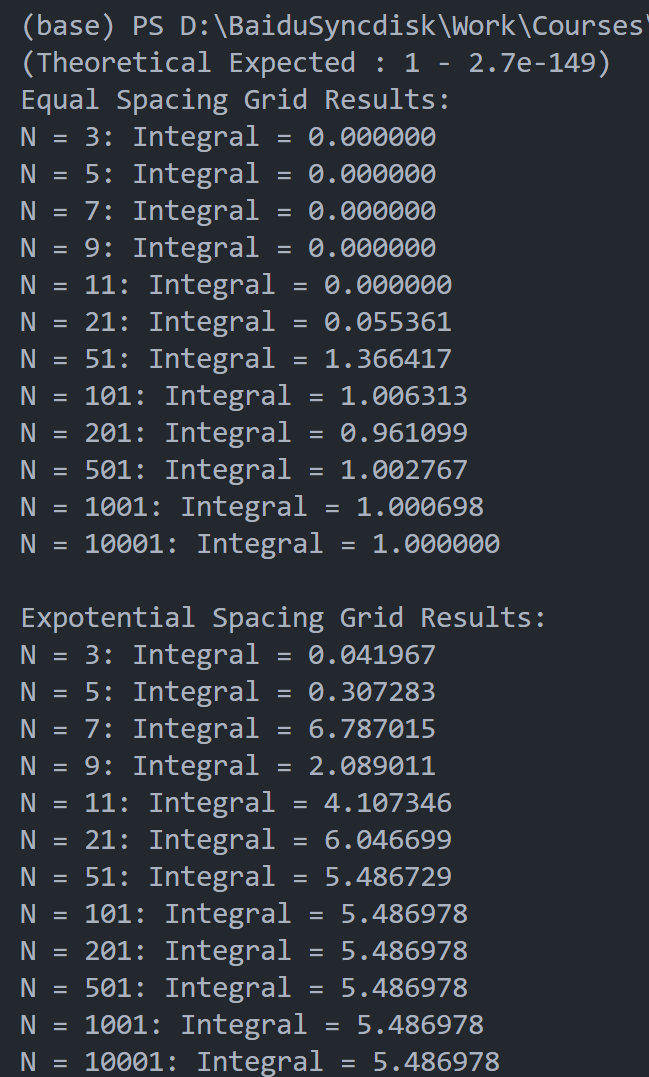
\includegraphics[width=1.0\textwidth]{Problem_1/figs/terminal.png}
    \caption{终端处理用户输入,此处均采用默认值}
\end{figure}
\begin{figure}[H]
    \centering
    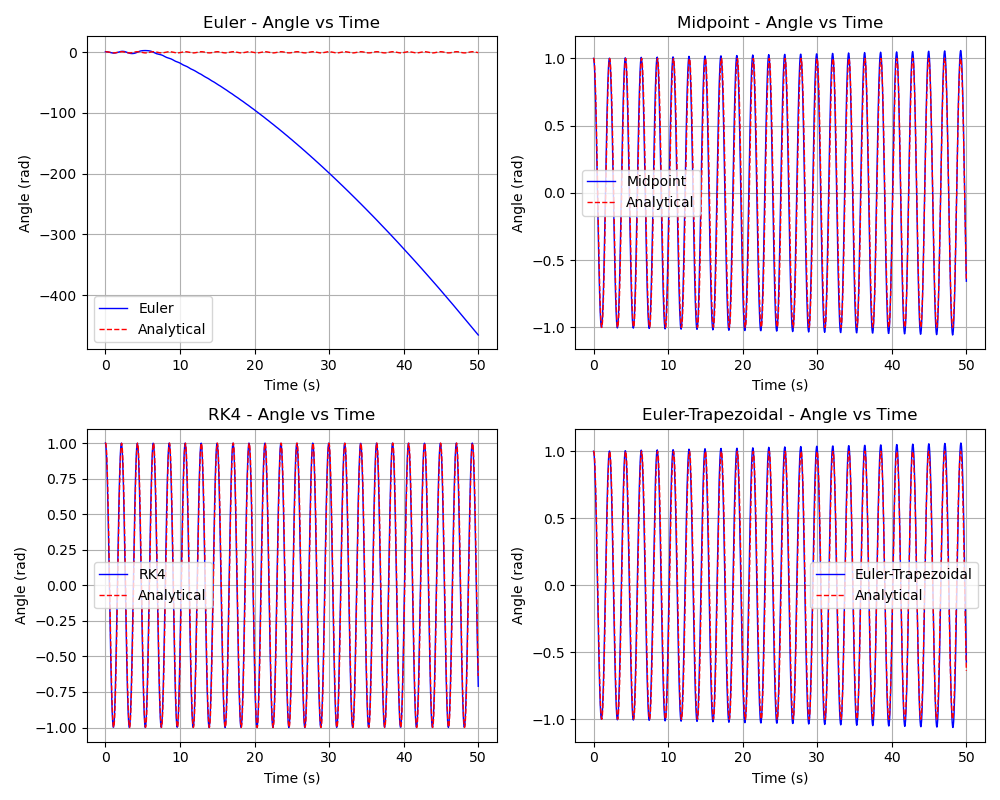
\includegraphics[width=1.0\textwidth]{Problem_1/figs/angle_time.png}
    \caption{角度随时间变化}
\end{figure}
\begin{figure}[H]
    \centering
    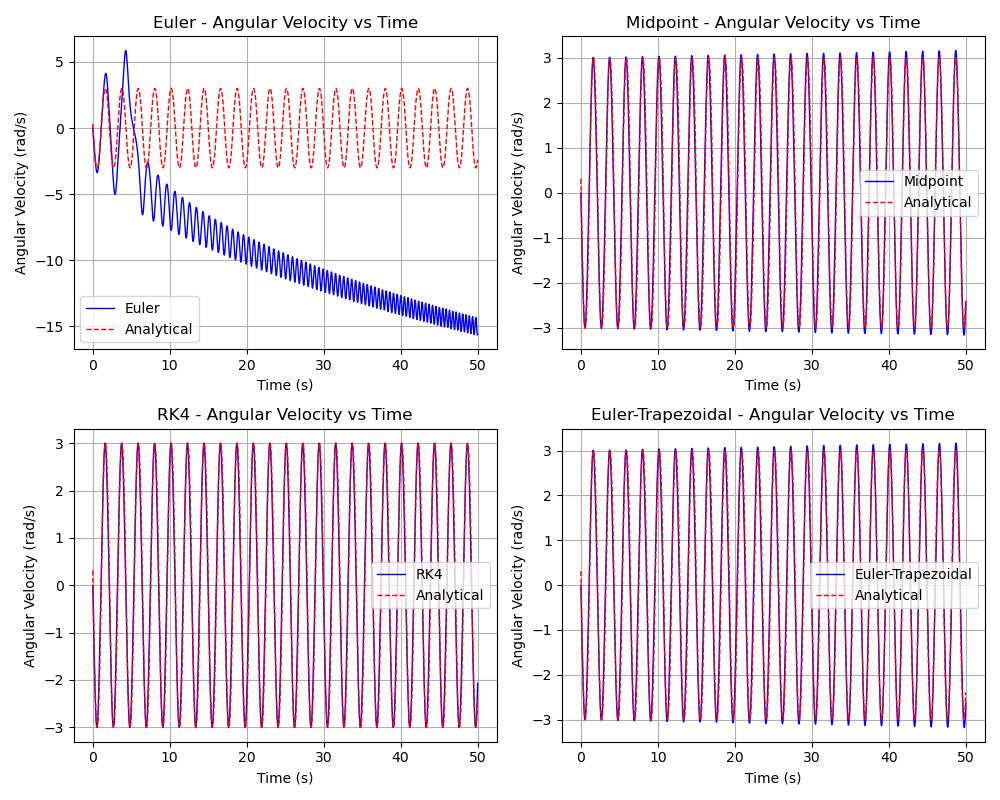
\includegraphics[width=1.0\textwidth]{Problem_1/figs/angle_velocity_time.png}
    \caption{角速度随时间变化}
\end{figure}
\begin{figure}[H]
    \centering
    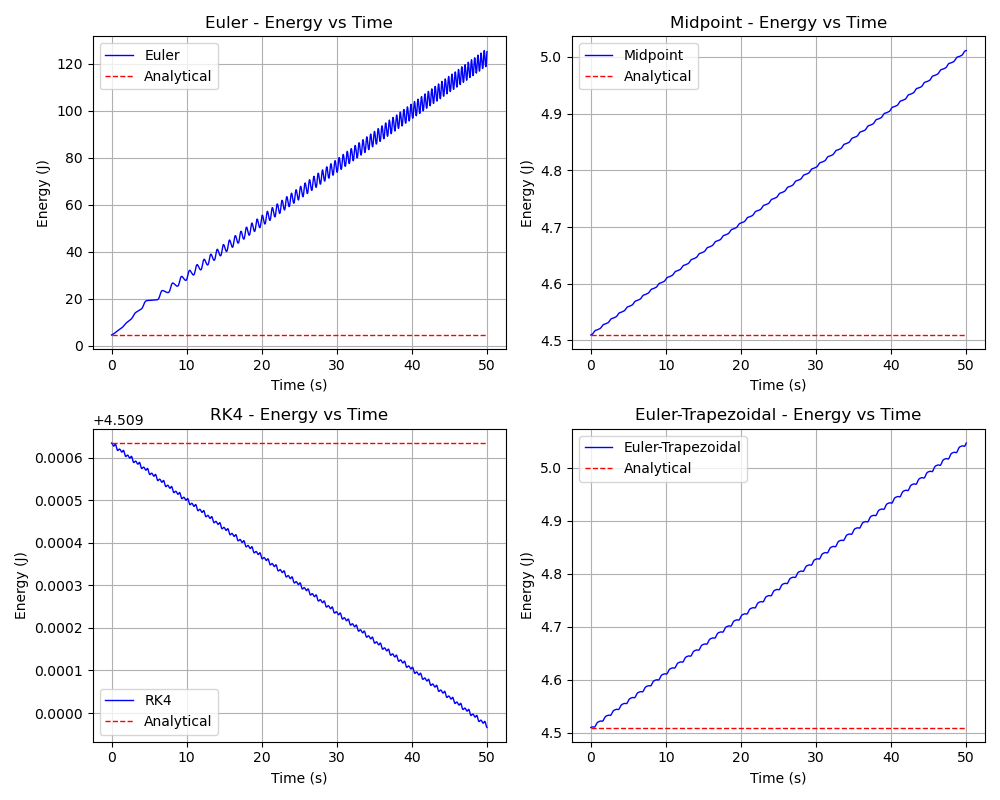
\includegraphics[width=1.0\textwidth]{Problem_1/figs/energy_time.png}
    \caption{能量随时间漂移}
\end{figure}
\begin{figure}[H]
    \centering
    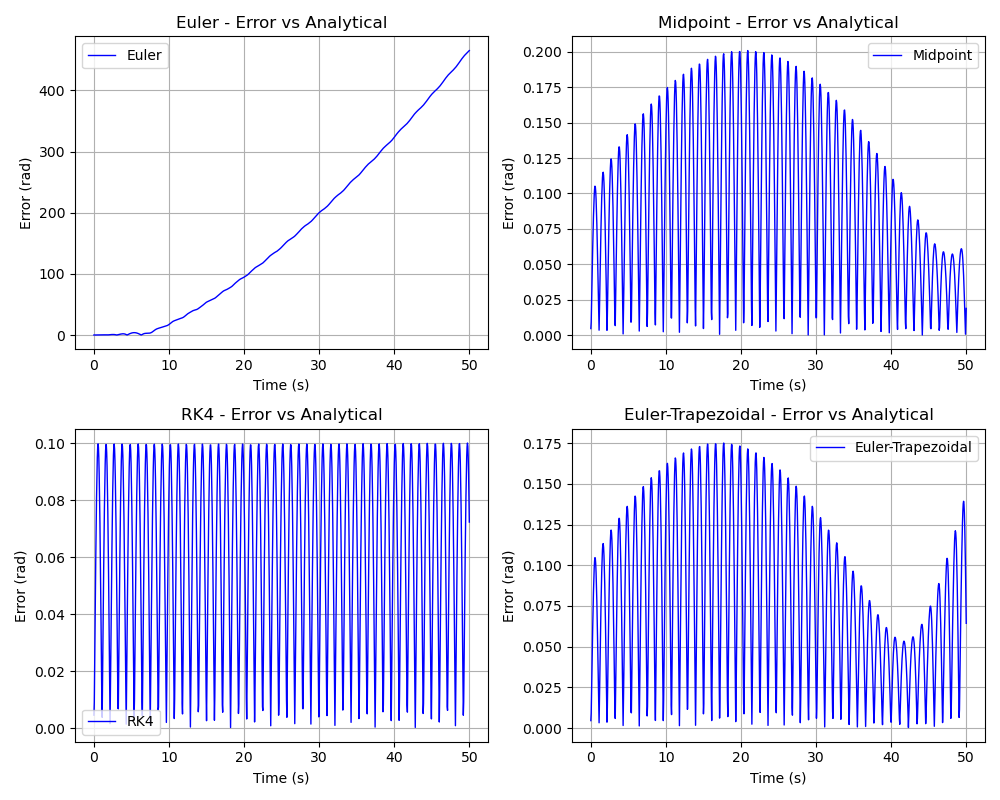
\includegraphics[width=1.0\textwidth]{Problem_1/figs/angle_error_time.png}
    \caption{角度与解析解误差随时间变化}
\end{figure}
可以看出,四种方法对比中,RK4方法的能量漂移最小,角度与角速度误差也最小。中点法与欧拉-梯形法次之,虽然角度、角速度误差在长时间后才逐渐显现,但能量漂移较大。欧拉法误差最大,一段时间后就崩溃。综上,RK4方法最为精确且稳定。

\section{题目 2:太阳黑子周期性检测}
\subsection{题目描述}
\noindent Write a code to numerically solve the radial Schrödinger equation for
\[
\left[-\frac{1}{2}\nabla^2+V(\mathbf{r})\right]\psi(\mathbf{r})=E\psi(\mathbf{r}), \quad V(\mathbf{r})=V(r)
\]
\begin{enumerate}
    \item \( V(r) = \frac{1}{r} \) (hydrogen atom)
    \item Considering the following potential:
    \[
    V(r) = -\frac{Z_{\text{ion}}}{r}\text{erf}\left(\frac{r}{\sqrt{2} r_{\text{loc}}}\right) 
    + \exp \left[ -\frac{1}{2} \left(\frac{r}{r_{\text{loc}}}\right)^{\frac{1}{2}}\right]
    \times \left[C_1 + C_2\left(\frac{r}{r_{\text{loc}}}\right)^2+C_3\left(\frac{r}{r_{\text{loc}}}\right)^4+C_4\left(\frac{r}{r_{\text{loc}}}\right)^6\right]
    \]
\end{enumerate}
where \(\text{erf}\) is the error function. And for Li, you could set:
\begin{itemize}
    \item \( Z_{\text{ion}}=3 \)
    \item \( r_{\text{loc}}=0.4 \)
    \item \( C_1=-14.0093922 \)
    \item \( C_2=9.5099073 \)
    \item \( C_3=-1.7532723 \)
    \item \( C_4=0.0834586 \)
\end{itemize}
\noindent Compute and plot the first three eigenstates. You could find more information about 'how to solve radial Schrödinger equation' and 'use of non-uniform grid (optional)' in the PPT.

\textbf{Special Note:} You may call any library functions for diagonalization.


\subsection{程序描述}

\subsection{伪代码}
Powered by \href{https://chatgpt.com/g/g-xJJAA2awf-latex-pseudocode-generator}{\LaTeX \ pseudocode generator}

\subsection{结果示例}



\end{document}